\title{Comparing Testability and Code Quality in Software Paradigms}
\author{
        Marc Coquand\\
        Department of Computer Science\\
        Umeå University\\
}
\date{\today}


\documentclass[12pt]{article}
\usepackage{listings}
\usepackage{amsthm}
\usepackage[utf8]{inputenc}
\usepackage[english]{babel}
\usepackage{tikz}
\usetikzlibrary{arrows}
\usepackage{romande}
\usepackage[T1]{fontenc}
\usepackage{float}

\theoremstyle{definition}
\newtheorem*{definition}{Definition}

\theoremstyle{theorem}
\newtheorem*{theorem}{Theorem}

\lstdefinestyle{customc}{
	belowcaptionskip=1\baselineskip,
	breaklines=true,
	frame=L,
	xleftmargin=\parindent,
	language=C,
	showstringspaces=false,
	basicstyle=\footnotesize\ttfamily,
	keywordstyle=\bfseries\color{green!40!black},
	commentstyle=\itshape\color{purple!40!black},
	identifierstyle=\color{blue},
	stringstyle=\color{orange},
}
\lstdefinestyle{customasm}{
	belowcaptionskip=1\baselineskip,
	frame=L,
	xleftmargin=\parindent,
	language=[x86masm]Assembler,
	basicstyle=\footnotesize\ttfamily,
	commentstyle=\itshape\color{purple!40!black},
}
\lstset{escapechar=@,style=customc}

\begin{document}
\maketitle

\begin{abstract} 

    This study's goal is to compare approaches to functional programs and
    object-oriented programs to find how it affects maintainability and code
    quality.  By looking at 3 cases, we analyze, how does a functional approach
    to software architecture compare to an OOP (Object-oriented programming)
    approach when it comes to maintainability and code quality?

\end{abstract}

\section{Introduction}
This is time for all good men to come to the aid of their party!


\section{Theory}\label{theory}

\subsection{Characteristics of Functional Programming}
Expressions and functions

\subsubsection{Iterator pattern}

\subsection{Object Oriented Programming}\label{oop}
Uses variables, commands and procedures

\subsubsection{SOLID principles}

\section{Methods}\label{methods}

\subsection{Measuring testability: Cyclomatic Complexity}\label{cyclomaticcomplexity}

Cyclomatic complexity is a complexity measure that looks to measure the amount
of paths through a program. The Cyclomatic complexity is an upper bound for the
number of test cases required for branch coverage of the code. 

\theoremstyle{definition}
\begin{definition}
The cyclomatic number $v(G)$ of a graph G with $n$ vertices, $e$ edges and $p$
connected components is $v(G) = e - n + p$.
\end{definition}

\begin{theorem}
In a strongly connected graph $G$, the cyclomatic number is equal to the
maximum number of linearly independent circuits.~\cite{McCabe}
\end{theorem}

Informally, we can think of cyclomatic complexity as a way to measure the amount
tests a program needs to reach full branch coverage. We construct a graph that
branches out based on when the control flow in our source code branches out. For
example given \texttt{f(bool) = if bool then 1; else 2}. To test
\texttt{f} we would need two tests, one where the if statement is false and one
where true, so the cyclomatic complexity is 2. We represent that as two
different edges in the graph. In summary the nodes of the graph represents
processing tasks and edges represent control flow between the nodes. 

\begin{figure}[H]
    \begin{lstlisting}
i = 0;
n=4; //N-Number of nodes present in the graph

while (i<n-1) do
j = i + 1;

while (j<n) do

if A[i]<A[j] then
swap(A[i], A[j]);

end do;
i=i+1;

end do; 
    \end{lstlisting}
    \caption{Example for cyclomatic complexity.}\label{c1excode}
\end{figure}

If we have the code found in example figure~\ref{c1excode}. To calculate the
complexity of this function we first construct a graph as seen in
figure~\ref{fig:c1exgraph}. From the graph we find $n=9, e=7, p=2\Rightarrow
v(G)=e-n+p=9-7+2=4$ is the cyclomatic number.

\begin{figure}[H]
    \centering
    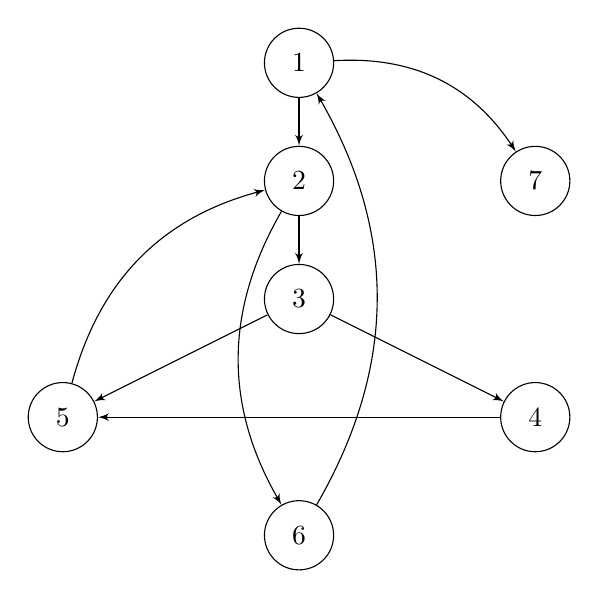
\begin{tikzpicture}
        \tikzset{vertex/.style = {shape=circle,draw,minimum size=2.5em}};
        \tikzset{edge/.style = {->,> = latex'}};
        \node[vertex] (a) at (3,6) {1};
        \node[vertex] (b) at (3,4.5) {2};
        \node[vertex] (c) at (3,3) {3};
        \node[vertex] (d) at (6,1.5) {4};
        \node[vertex] (e) at (0, 1.5) {5};
        \node[vertex] (f) at (3,0) {6};
        \node[vertex] (g) at (6,4.5) {7};
        \draw[edge] (a)  to  (b);
        \draw[edge] (a)  to[bend left]  (g);
        \draw[edge] (b)  to (c);
        \draw[edge] (b)  to[bend right] (f);
        \draw[edge] (c)  to (d);
        \draw[edge] (c)  to (e);
        \draw[edge] (d)  to (e);
        \draw[edge] (e)  to[bend left] (b);
        \draw[edge] (f)  to[bend right] (a);
    \end{tikzpicture}
    \caption{Cyclomatic complexity graph for figure~\ref{c1excode}}\label{fig:c1exgraph}
\end{figure}

\subsubsection{Cyclomatic Complexity in Functional Programming}

The definition of cyclomatic complexity in Section~\ref{cyclomaticcomplexity} is
not ideal for functional programming. Cyclomatic complexity is calculated by
creating graphs based on control flow operations such as while loops and if
statements. In functional programming everything is a function, thus the
cyclomatic complexity will always tend to 0 using this definition. So we define a
different method of calculating the cyclomatic complexity for functional
programs. 

\theoremstyle{definition}
\begin{definition}
    The cyclomatic complexity number, in functional programming, for a function
    is equal to 1 plus the sum of the left hand side, called LHS, plus the sum
    of the right hand side, called RHS. RHS is the sum of the number of guards,
    logical operators, filters in a list comprehension and the pattern
    complexity in a list comprehension. LHS is equal to the pattern complexity
    of LHS. The pattern complexity is equal to the number of identifiers in the
    pattern, minus the number of unique identifiers in the pattern plus the
    number of arguments that are not identifiers. 
\end{definition}

Instead of cyclomatic graphs we instead construct flowgraphs, such as the one
seen in Figure~\ref{fig:cyclomaticfunctional} to model the function.

\begin{figure}[H]
    \begin{lstlisting}
    split :: (a -> Bool) -> [a] -> ([a], [a])
    split onCondition [] = ([], [])
    split onCondition (x:xs) =
        let 
            (ys, zs) = split onCondition xs
        in 
            if (onCondition x) then 
                (x:ys, zs)
            else 
                (ys, x:zs)
    \end{lstlisting}
    \caption{Recursively split a list into two based on a given condition in
    Haskell. For example \texttt{split (>3) [1,2,3,4,5] =
    ([4,5],[1,2,3])}.}\label{fig:split}
\end{figure}

For example, given the Haskell code in Figure~\ref{fig:split}. To calculate LHS
we find three pattern identifiers which are $onCondition$, $x$ and $xs$, there
are two unique pattern identifiers which are $x$ and $xs$, and there are two non
identifiers which are $[]$ and $(:)$.

We do not count the $otherwise$ clause, similar to how we do not count the
$else$ statement in normal procedural cyclomatic complexity.~\cite{bergklaas}


\begin{figure}[H]
    \centering
    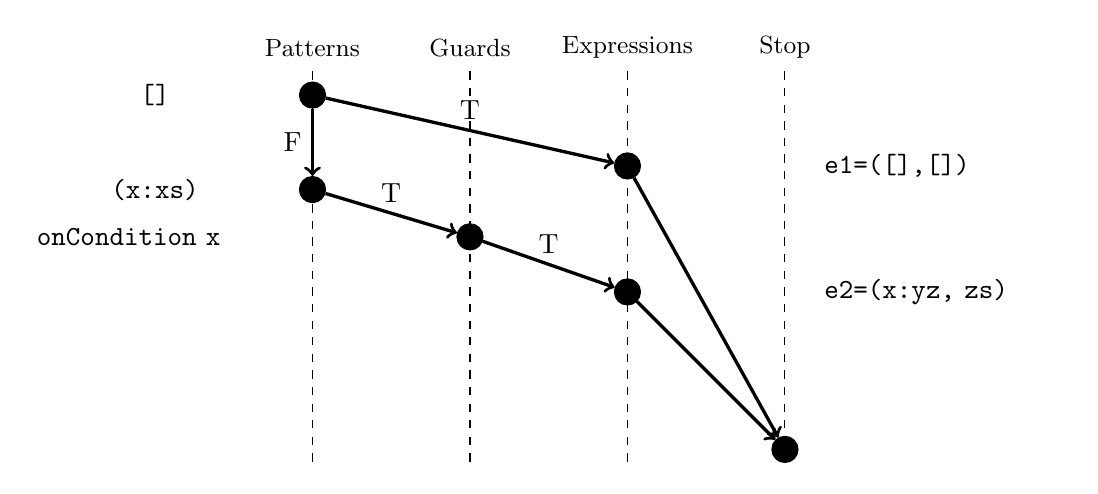
\begin{tikzpicture}
        \tikzset{vertex/.style = {shape=circle,fill=black,draw,minimum size=0.01em}};
        \draw[dashed] (0,0) -- (0,-5) (2,0) -- (2,-5) (4, 0) -- (4, -5) (6, 0)
        -- (6, -5);
        \node at (0,.3) {\small{Patterns}};
        \node at (2,.3) {\small{Guards}};
        \node at (4,.3) {\small{Expressions}};
        \node at (6,.3) {\small{Stop}};
        \node[vertex] (a) at (0,-0.3) {};
        \node at (-2,-0.3) {\texttt{[]}};
        \node[vertex] (b) at (4,-1.2) {};
        \draw[->, very thick] (a) to node [above] (TextNode) {T} (b) ;
        \node[vertex] (c) at (0,-1.5) {};
        \node at (-2,-1.5) {\texttt{(x:xs)}};
        \draw[->, very thick] (a) to node [left] (TextNode) {F} (c) ;
        \node[align=left, text width=3cm] at (8,-1.2) {\texttt{e1=([],[])}};
        \node[vertex] (d) at (2,-2.1) {};
        \draw[->, very thick] (c) to node [above] (TextNode) {T} (d) ;
        \node[align=left, text width=3cm] at (-2,-2.1) {\texttt{onCondition x}};
        \node[vertex] (e) at (4,-2.8) {};
        \draw[->, very thick] (d) to node [above] (TextNode) {T} (e) ;
        \node[align=left, text width=3cm] at (8,-2.8) {\texttt{e2=(x:yz, zs)}};
        \node[vertex] (g) at (6,-4.8) {};
        \draw[->, very thick] (e) to (g) ;
        \draw[->, very thick] (b) to (g) ;
    \end{tikzpicture}
    \label{fig:cyclomaticfunctional}
    \caption{Flowgraph for split.}
\end{figure}

\subsection{Cognitive Dimensions}

\subsection{Case studies}

\subsubsection{Simplified chess game}

Chess is a famous game and assumed that the reader know how it works. Aim
is to implement a simplified variant of it. This is not ordinary chess but a
simplified version:

\begin{itemize} 
    \item Only pawns and horses exist.
    \item You win by removing all the other players pieces.
\end{itemize}

The player should be able to do the following:

\begin{itemize} 
    \item List all available moves for a certain chess piece. 
    \item Move the chess piece to a given space
    \item Switch player after move
    \item Get an overview of the board
    \item Get an error when making invalid moves
\end{itemize}

\subsubsection{to-do List}

A common task in programming is to create some kind of data store with
information. A to-do list is a minimal example of that. It consists of a list of
items that can be used to remember what to do later. The user should be able to:

\begin{itemize}
    \item Create a new item in the to-do list.
    \item Remove an item from the to-do list.
    \item See all items in the to-do list.
    \item Update an item from the to-do list.
\end{itemize}

\subsubsection{Chatbot engine}

Oftentimes when developing applications we have to deal with complex information
input. One of those cases is when we have chat bots. Chat bots are interactive
programs that respond with a text answer to the users input. For this
application we will implement the following:

\begin{itemize}
    \item Interpretor that can handle semi-complex inputs and deal with errors.
    \item Give answers to those inputs in form of text messages.
\end{itemize}    

\section{Results}\label{results}
We worked so hard, yet achieved very little.

\section{Limitations}\label{limitations}

\subsection{Improvements to implementation}

\bibliographystyle{abbrv}
\bibliography{thesis}

\end{document}
